\chapter{Genetic Algorithm}
\label{chapter:intro}
\section{簡介}
遺傳演算法(Genetic Algorithm,GA)是一種從遺傳科學中獲得啟發的技術,目前被廣泛應用於解決優化問題,尤其在特徵篩選方面。在GA中通常使用染色體的概念作為解決方案,通常基因數與特徵數相等,例如 \(Z=(0,1,1,0,1,0,0,0)\) 代表一染色體上共有8個特徵,1則代表以選擇特徵;0則代表未選擇特徵。
GA主要由三種運算組成,分別為親代選擇、交叉與突變。首先會生成具有隨機染色體集合的初始群集,之後評估每個染色體的適應度,並從適應度的概率來選擇親代父母,接下來在親代父母之間進行交叉配對,生成從親代父母繼承基因的染色體特徵子集,此外根據突變率可能導致生成的染色體子集突變(即0變1或是1變0),之後評估新生成的染色體子集適合度,並將新生成的染色體子集加入當前的群集中,並根據適合度進行排序,選擇最佳的N條染色體應用於下一代,重複該算法直到設定的最大迭代次數為止,最後選擇全局最佳染色體作為最佳特徵子集。
\begin{figure}[H]
	\centerline{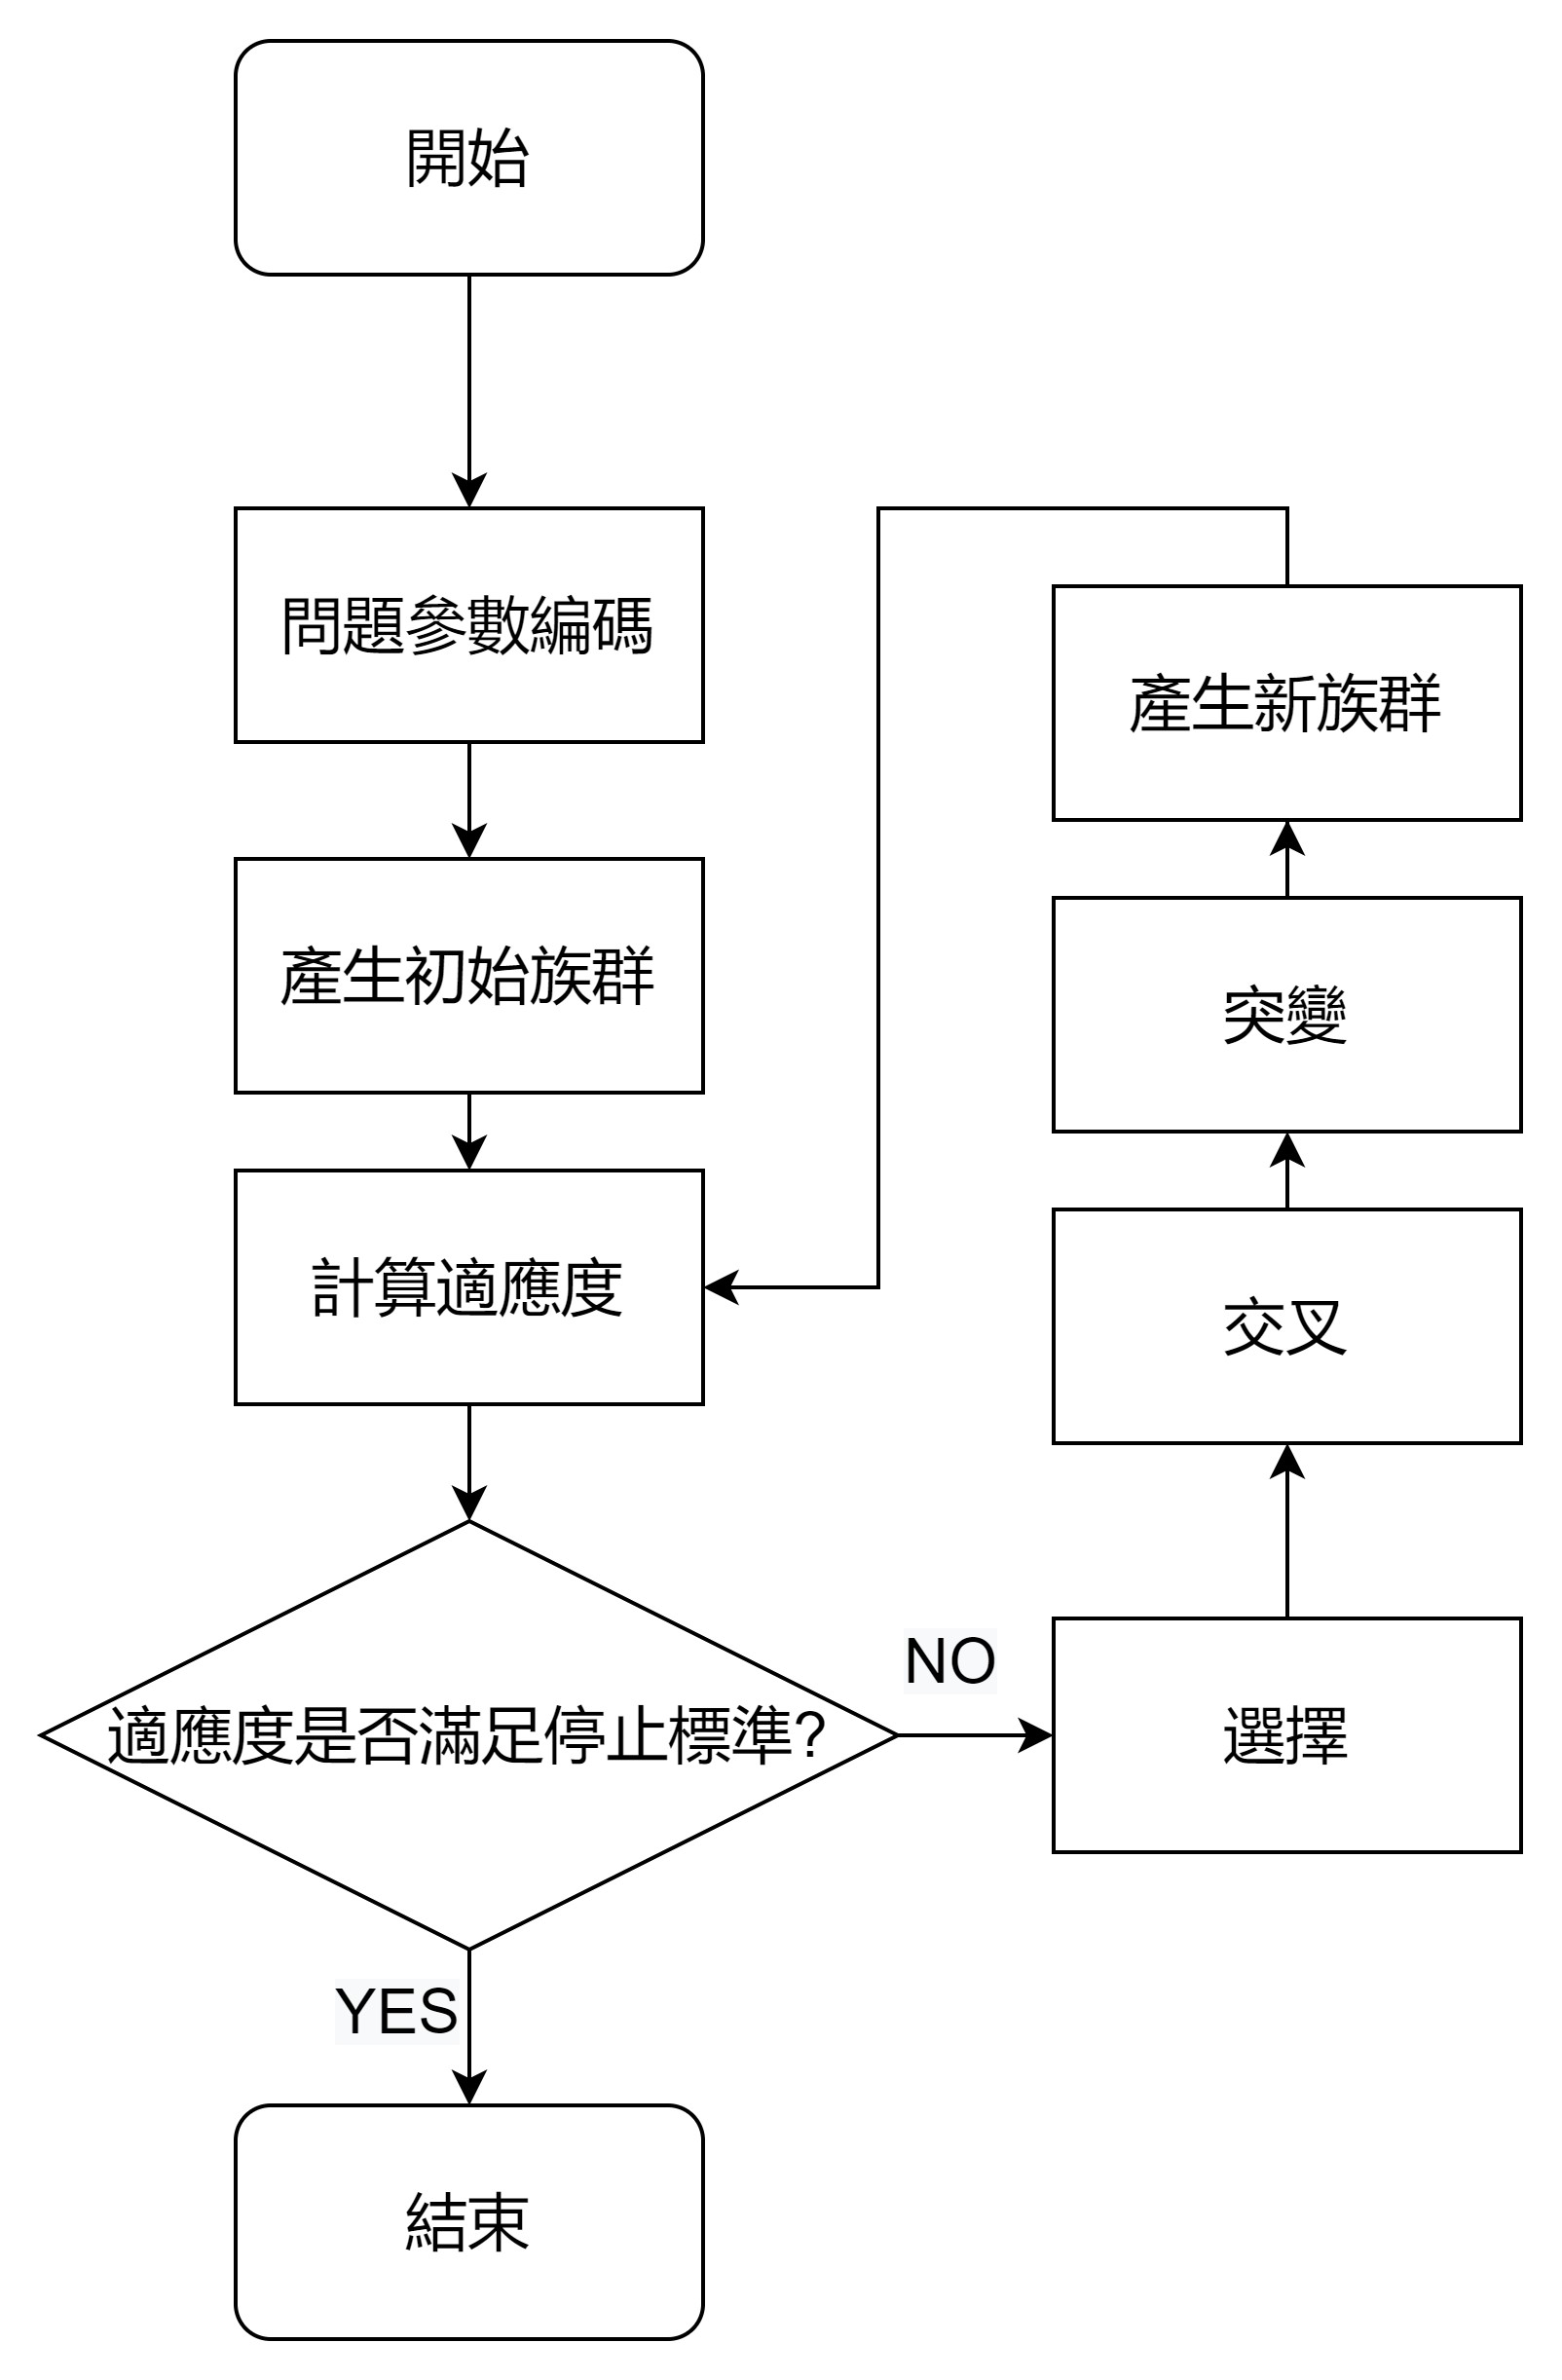
\includegraphics[height=8cm]{pic/GAFlowChart.PNG}}
	\caption{GA流程圖}
	\label{fig:GAFlowChart}
\end{figure}

\label{sec:background}
\section{參數編碼}
在使用GA來解決問題前,將資料編碼(Encode)成染色體,是基因演算法的關鍵議題,也是首要任務。其中常見的為二元編碼(Binary Encoding)。


%%如何將一個問題所需處理的資料編碼(Encode) 成染色體,是GA的一個關鍵議題,染色體編碼是要利用GA來解決問題時的首要任務。其中最常見的是用二元編碼 (Binary Encoding) 。

利用二元編碼 (Binary Encoding)時,會將選好的特徵基因進行排序,1 代表特徵被選擇;0 代表特徵未被選擇,假設一條染色體有五個特徵可以選擇,所構成的染色體從00000~11111共有32個可行解。

\section{適應度計算}

%%%在每完成初始族群取選後,須針對所有被選取的個體,計算其適應能力,做為接下來選種的依據, 每一個個體都被評估後得到一個適應能力值,族群中的個體被按照適應度排序,適應度高的在前面,如果用代價函數(Cost Function)來當評估標準,則需看實際問題是要求最大值(Maximum)還是最小值(Minimum)。

在產生新的族群後,會將所有被選取的個體,計算其適應能力,做為接下來選種的依據, 每個個體經過適應函數的評估後,會得到一個適應能力值,接著族群中的個體會照適應度排序,適應度高的在前面,適應度低的在 後面。
此外再進行適應度計算時,需考慮實際問題是要求最大值(Maximum)還是最小值(Minimum),作為適應函數制定的依據。

\section{親代選擇}
在這個階段中,GA會利用適應函數所評估出個體的適應度值,根據不同的選擇演算法進行優勝劣汰的操作。適應度較高的個體會被挑選出來,複製到下一代群體中的機率較大,適應度低的自然被選出來的機率就較小。 這樣可以使得群體中個體的適應度不斷的往最佳解的方向移動,而不是盲目搜尋。

\subsection{輪盤式選擇(Roulette Wheel Selection)}

藉由上個階段所得到每一個體的適應度,計算出此適應度在群體適應度總和中所佔的比例,表示該個體在選擇過程中會被選中的機率。
因此適應程度越好,所包含的面積就越大,被選擇的機率越大;適應程度越差,包含的面積就越小,被選擇的機率也因此越小。
如此以來,在選擇時適應程度越好的,也越有機會被選中,如同生物進化過程中的「適者生存,不適者淘汰」的概念,希望將優良基因會遺傳給下一代的個體。
如果群體的適應度差異巨大時,最佳個體的被選擇機率會大幅成長,容易使這個最佳個體充斥在當前群體中,使得群體喪失多樣性,過早失去進化能力。

\begin{table}[h!]
	\centering
	\label{tab:GeneEncodeAndFitness}
	\begin{tabular}{rrrr}
\toprule
  & 基因 & 適應度 & 百分比  \\
\midrule
  & 1001  & 5  & 6.5\%      \\
  & 1101  & 33  & 42.8\%      \\
  & 0100  & 10  & 13\%      \\
  & 0011  & 29  & 37.7\%      \\
\bottomrule
\end{tabular}

	\caption{基因編碼與適應度}
\end{table}

\begin{figure}[H]
	\centerline{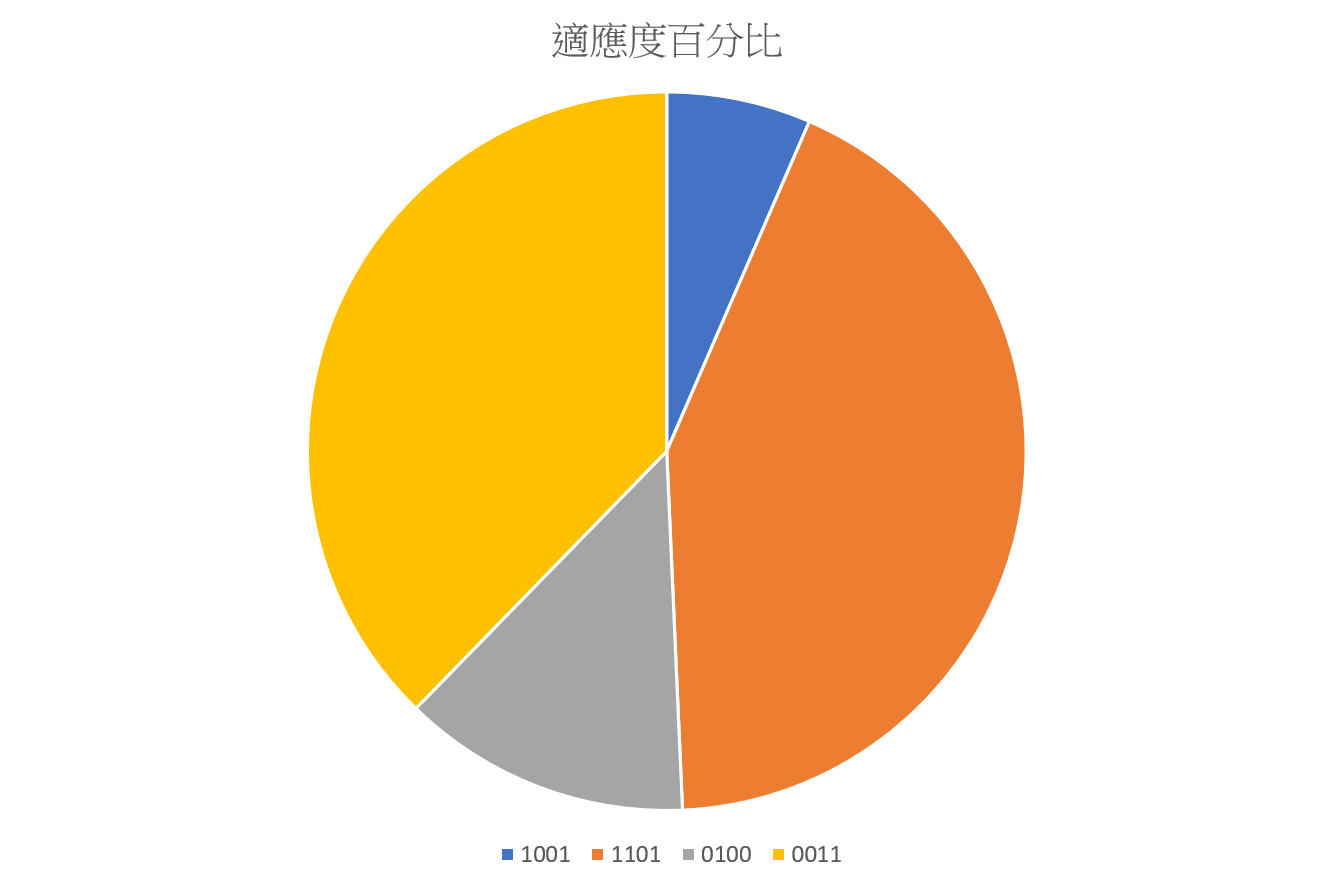
\includegraphics[width=10cm]{pic/wheelFitness.png}}
	\caption{輪盤法適應度百分比圖}
	\label{fig:WheelMethodPercentage}
\end{figure}


\subsection{競爭式選擇(Tournament Selection)}
按照輪盤選擇的機率為依據,隨機取得幾個基因序列,兩兩進行比較,將適應力較好的留下,如圖\ref{fig:TournamentSelection},其中紅色框框為經競爭留下的基因。此外,因為是用機率選取基因,所以不但可以塞選出好基因,也能避免輪盤法則的缺點發生。

\begin{figure}[H]
	\centerline{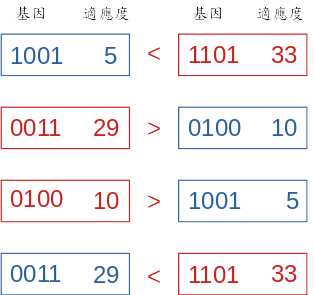
\includegraphics[width=6cm]{./pic/us1jJ97T.png}}
	\caption{競爭式選擇}
	\label{fig:TournamentSelection}
\end{figure}

\newpage
\section{交叉配對}
交叉配對(crossover)會將兩個親代的染色體基因進行重新組合分配,從而產生下一代個體的過程,通過交叉配對可以將兩個親代的優勢基因組合在一起,產生適應度更高、更接近最優解的新個體。

		\subsection{單點交叉}
	      單點交叉算法如圖\ref{fig:SinglePointCross},指定了單個交換點用於親代的基因交換重組。
	      \begin{figure}[H]
		      \centerline{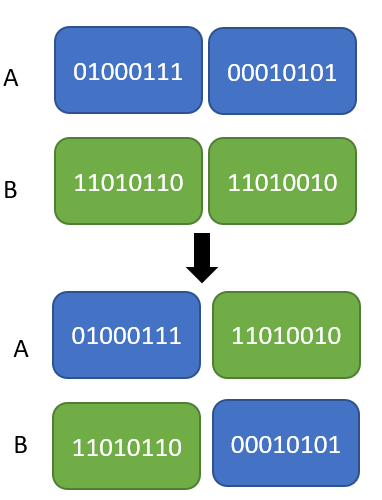
\includegraphics[height=6cm]{pic/one.PNG}}
		      \caption{單點交叉示意圖}
		      \label{fig:SinglePointCross}
	      \end{figure}

	      \subsection{多點交叉}
	      多點交叉算法如圖\ref{fig:MultiPointCross},指定了多個交換點用於父輩的基因交換重組。
	      \begin{figure}[H]
		      \centerline{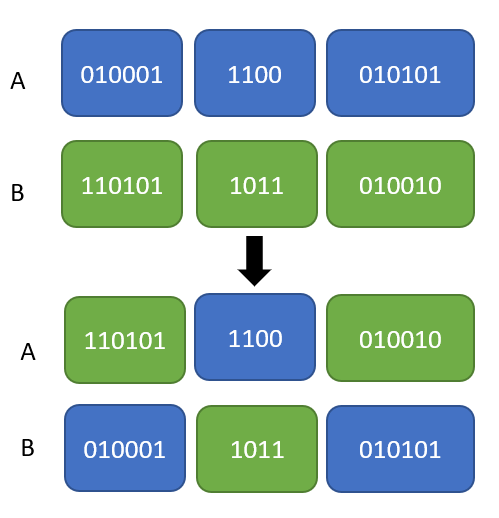
\includegraphics[height=6cm]{pic/TWO.PNG}}
		      \caption{多點交叉示意圖}
		      \label{fig:MultiPointCross}
	      \end{figure}

	      \subsection{均勻交叉}
	      單點交叉跟多點交叉,存在染色體中某些部分的基因會被過早地捨棄,為了避免這個問題,有了均勻交叉。在均勻交叉中如圖\ref{fig:avg},首先隨機選擇染色體上的交換位,然後隨機確定交換的基因是父輩染色體上交換位的前部分基因還是後部分基因,最後對父本染色體的基因進行重組從而產生新的下一代個體。
	      \begin{enumerate}[(a)]
		      \item
		            隨機產生一個與個體長度相同的遮蔽字串W(Mask String)。

		      \item
		            若W=0則相對應父輩基因保留;若W=1則相對應父輩基因進行交叉。
	      \end{enumerate}
	      \begin{figure}[H]
		      \centerline{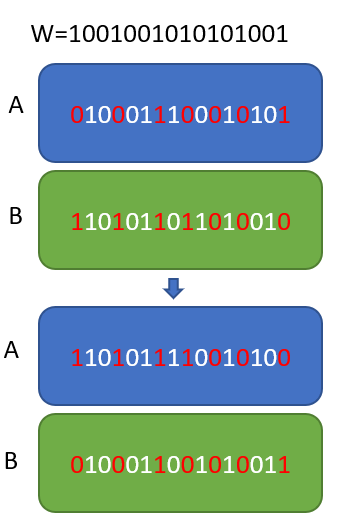
\includegraphics[height=6cm]{pic/AVG.PNG}}
		      \caption{均勻交叉示意圖W=1001001010101001}
		      \label{fig:avg}
	      \end{figure}






\section{突變}
突變是為了避免種群中的染色體過於相似,使算法陷入區域最佳解,減慢或停止進化過程。雖然遺傳算法利用交叉配對中,從全局角度尋找一些較好的個體編碼結構,有助於獲得問題的最佳解,但僅交配操作不能對搜索空間的細節進行局部搜索。這時,如果對個體編碼串中的一些基因值進行變異調整如圖\ref{fig:GAmut},個體可以從局部的角度更接近最佳解,從而提高遺傳算法的局部搜索能力。

\begin{figure}[H]
	\centerline{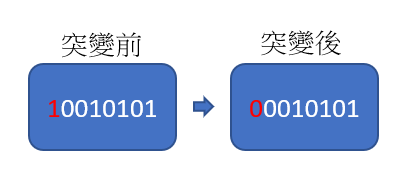
\includegraphics[height=2.5cm]{pic/GAmut.PNG}}
	\caption{突變示意圖}
	\label{fig:GAmut}
\end{figure}
